% Автоматаар үүсгэсэн — эх файл: README.md
\chapter{Гарын авлагын танилцуулга}

\hypertarget{ux43bux430ux431ux43eux440ux430ux442ux43eux440ux438ux439ux43d-ux430ux436ux43bux44bux43d-ux441ux430ux43d-raspberry-pi-3b-ux445ux443ux432ux438ux43bux431ux430ux440}{%
\section{Лабораторийн ажлын сан · Raspberry Pi 3B хувилбар}\label{ux43bux430ux431ux43eux440ux430ux442ux43eux440ux438ux439ux43d-ux430ux436ux43bux44bux43d-ux441ux430ux43d-raspberry-pi-3b-ux445ux443ux432ux438ux43bux431ux430ux440}}

Энэ сан нь CNC302 хичээлийн \textbf{найман лабораторийн ажлыг} агуулна. Найман лаборатори нь тус тусдаа биш --- \textbf{нэг ажиллаж буй платформыг үе шаттай өргөтгөж бүтээнэ}. Лаборатори бүрийн эцэст таны систем ажиллагаатай хэвээр байх ёстой бөгөөд дараагийн лаборатори үүн дээр үргэлжилнэ.

\hypertarget{ux445ux43eux451ux440-ux434ux430ux432ux445ux430ux440ux433ux430ux442-ux430ux436ux43bux44bux43d-ux43eux440ux447ux438ux43d}{%
\section{1. Хоёр давхаргат ажлын орчин}\label{ux445ux43eux451ux440-ux434ux430ux432ux445ux430ux440ux433ux430ux442-ux430ux436ux43bux44bux43d-ux43eux440ux447ux438ux43d}}

Энэ курсын гол архитектурын шийдэл: \textbf{үүл ба ирмэгийг ХОЁР ӨӨР ТӨХӨӨРӨМЖ дээр} ажиллуулна.

\begin{figure}
\centering
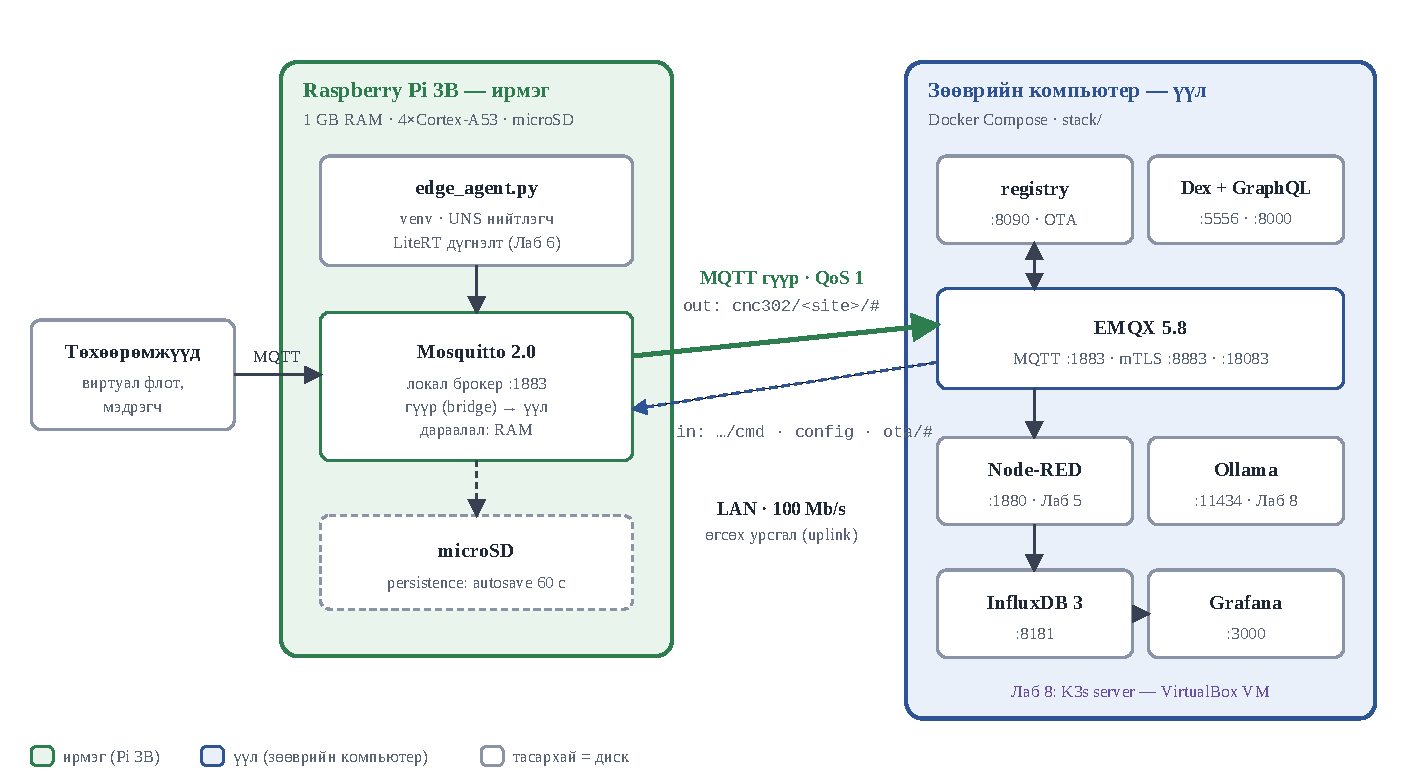
\includegraphics{figures/fig-architecture.pdf}
\caption{Зураг 0.1 --- Хоёр давхаргат архитектур: зөөврийн компьютер (үүл) ба Raspberry Pi 3B (ирмэг), хооронд нь MQTT гүүр}
\end{figure}

\begingroup\scriptsize\begin{longtable}[]{@{}
  >{\raggedright\arraybackslash}p{(\columnwidth - 4\tabcolsep) * \real{0.3333}}
  >{\raggedright\arraybackslash}p{(\columnwidth - 4\tabcolsep) * \real{0.3333}}
  >{\raggedright\arraybackslash}p{(\columnwidth - 4\tabcolsep) * \real{0.3333}}@{}}
\toprule
\begin{minipage}[b]{\linewidth}\raggedright
Төхөөрөмж
\end{minipage} & \begin{minipage}[b]{\linewidth}\raggedright
Үүрэг
\end{minipage} & \begin{minipage}[b]{\linewidth}\raggedright
Юу ажиллах
\end{minipage} \\
\midrule
\endhead
\bottomrule
\endlastfoot
\textbf{Оюутны зөөврийн компьютер} & \textbf{Үүлний давхарга} (IoT лавлах архитектурын 3-р давхарга) & EMQX, InfluxDB, Grafana, төхөөрөмжийн бүртгэл, Node-RED, GraphQL API, Dex, Ollama \\
\textbf{Raspberry Pi 3B} & \textbf{Ирмэгийн давхарга} (2--3-р давхаргын зааг) & Mosquitto брокер + үүл рүү гүүр, ирмэгийн агент, LiteRT (TFLite) дүгнэлт, Лаб 8-д K3s agent (server нь зөөврийн компьютер дээрх VM) \\
\end{longtable}\endgroup

\hypertarget{ux44fux430ux433ux430ux430ux434-ux445ux443ux432ux430ux430ux441ux430ux43d-ux431ux44d}{%
\subsection{Яагаад хуваасан бэ}\label{ux44fux430ux433ux430ux430ux434-ux445ux443ux432ux430ux430ux441ux430ux43d-ux431ux44d}}

Raspberry Pi 3B-ийн албан ёсны техникийн үзүүлэлт ба үр дагавар:

\begingroup\scriptsize\begin{longtable}[]{@{}
  >{\raggedright\arraybackslash}p{(\columnwidth - 4\tabcolsep) * \real{0.3333}}
  >{\raggedright\arraybackslash}p{(\columnwidth - 4\tabcolsep) * \real{0.3333}}
  >{\raggedright\arraybackslash}p{(\columnwidth - 4\tabcolsep) * \real{0.3333}}@{}}
\toprule
\begin{minipage}[b]{\linewidth}\raggedright
Үзүүлэлт
\end{minipage} & \begin{minipage}[b]{\linewidth}\raggedright
Утга
\end{minipage} & \begin{minipage}[b]{\linewidth}\raggedright
Үр дагавар
\end{minipage} \\
\midrule
\endhead
\bottomrule
\endlastfoot
Санах ой & \textbf{1 GB} (OS-д харагдах \texttt{MemTotal}-ийг Лаб 1-д хэмжинэ) & ThingsBoard-ын албан ёсны заавар хөгжүүлэлтэд ч 4 GB RAM шаарддаг --- огт багтахгүй \\
Процессор & BCM2837, 4 × Cortex-A53 (Armv8) @ 1.2 GHz & JVM-т суурилсан платформ хэт удаан \\
Сүлжээ & \textbf{100 Mb/s} Ethernet; 4 × USB 2.0 & Өгсөх урсгал (uplink) 100 Mb/s-ээр хязгаарлагдана \\
Диск & \textbf{зөвхөн microSD} & persistence, swap бичилт удаан (Лаб 5-д хэмжинэ) \\
Өргөтгөл & \textbf{PCIe байхгүй} & Raspberry Pi AI Kit (Hailo) нь Raspberry Pi 5-д зориулагдсан --- боломжгүй \\
\end{longtable}\endgroup

Гэхдээ энэ бол зөвхөн хязгаарлалт биш. Бодит үйлдвэрлэлийн IoT систем яг \textbf{ийм} байдаг: хүчирхэг үүл, сул ирмэг, хооронд нь найдваргүй холбоос. Pi 5 дээр бүгдийг нэг дор ажиллуулах нь илүү тохилог боловч \textbf{Edge--Fog--Cloud континуумыг заахгүй}. Pi 3B үүнийг заахаас өөр аргагүй болгоно:

\begin{itemize}
\tightlist
\item
  Гүүр (bridge) яагаад хэрэгтэйг \textbf{холбоос тасарч үзсний дараа} ойлгоно (Лаб 5)
\item
  Ирмэг дээрх дүгнэлт яагаад хэрэгтэйг \textbf{өгсөх урсгалыг (uplink) хэмнэж үзсний дараа} ойлгоно (Лаб 6)
\item
  Санах ойн төсөв яагаад чухлыг \textbf{OOM-той тулгарсны дараа} ойлгоно (Лаб 1)
\end{itemize}

\begin{quote}
\textbf{Зарчим:} Хүнд зүйл \textbf{үүл} дээр, хурдан хариу шаардсан зүйл \textbf{ирмэг} дээр. Аль ч алхмыг эхлэхийн өмнө "энэ хаана ажиллах ёстой вэ?" гэж асуу. Заавар бүрийн алхам бүрд {[}ЗК{]} (зөөврийн компьютер) эсвэл {[}Pi{]} (Pi) тэмдэглэгээ байна.
\end{quote}

\hypertarget{ux441ux430ux43dux433ux438ux439ux43d-ux431ux4afux442ux44dux446}{%
\section{2. Сангийн бүтэц}\label{ux441ux430ux43dux433ux438ux439ux43d-ux431ux4afux442ux44dux446}}

\begin{verbatim}
CNC302-labs/
├── README.md              ← энэ файл
├── SETUP.md               ← Лаб 1-ээс өмнө нэг удаа хийх бэлтгэл
│
├── stack/                 [ЗК] ҮҮЛ — зөөврийн компьютер дээр
│   ├── docker-compose.yml       ← ЖИВЭЭ ФАЙЛ, лаборатори бүрт өснө
│   ├── docker-compose.tb.yml    ← ThingsBoard (сонголтот харьцуулалт)
│   ├── docker-compose.influx2.yml  ← InfluxDB 2.7 нөөц хувилбар
│   ├── .env.example
│   └── Makefile
│
├── edge/                  [Pi] ИРМЭГ — Raspberry Pi 3B дээр
│   ├── docker-compose.yml       ← mosquitto
│   ├── mosquitto/
│   │   ├── mosquitto.conf
│   │   └── conf.d/bridge.conf.template   ← `make bridge` үүсгэнэ
│   ├── agent/
│   │   ├── edge_agent.py        ← ирмэгийн агент
│   │   ├── Dockerfile           ← Лаб 8-д K3s agent-д (компьютер дээр arm64-д барина)
│   │   └── cnc302-edge-agent.service
│   ├── .env.example
│   └── Makefile
│
├── tools/                 бүх лабораторид хэрэглэгдэх хэрэгслүүд
│   ├── sim_device.py            ← виртуал төхөөрөмжийн флот
│   ├── qos_latency.py           ← QoS × зам (loopback/LAN/bridge) саатал
│   └── measure_stack.sh         ← --role edge|cloud
│
├── lab01/ … lab08/        лаборатори бүрийн заавар ба ажлын файлууд
│   ├── README.md                ← ЗААВАР
│   ├── *.py *.sh
│   └── out/                     ← гаралт (.gitignore-д)
│
└── docs/
    ├── report-template.md
    ├── troubleshooting.md
    └── resource-budget.md       ← 1 GB-ын арифметик
\end{verbatim}

\hypertarget{stack-ux431ux430-edge-ux444ux43eux43bux434ux435ux440ux44bux43d-ux434ux4afux440ux44dux43c}{%
\subsection{\texorpdfstring{\texttt{stack/} ба \texttt{edge/} фолдерын дүрэм}{stack/ ба edge/ фолдерын дүрэм}}\label{stack-ux431ux430-edge-ux444ux43eux43bux434ux435ux440ux44bux43d-ux434ux4afux440ux44dux43c}}

\texttt{stack/\allowbreak{}docker-compose.\allowbreak{}yml} болон \texttt{edge/\allowbreak{}docker-compose.\allowbreak{}yml} бол \textbf{таны багийн живээ файлууд}. Лаборатори бүрт та тэдгээр рүү үйлчилгээ нэмж, тохиргоо өөрчилнө. Эвдэрсэн бол Git-ийн түүхээс сэргээнэ:

\begin{Shaded}
\begin{Highlighting}[]
\FunctionTok{git}\NormalTok{ log }\AttributeTok{{-}{-}oneline} \AttributeTok{{-}{-}}\NormalTok{ stack/docker{-}compose.yml}
\FunctionTok{git}\NormalTok{ checkout }\OperatorTok{\textless{}}\NormalTok{commit}\OperatorTok{\textgreater{}}\NormalTok{ {-}{-} stack/docker{-}compose.yml}
\end{Highlighting}
\end{Shaded}

Тиймээс \textbf{лаборатори бүрийн эцэст commit хийх} нь зөвхөн үнэлгээний шаардлага биш, өөрийн даатгал юм.

\hypertarget{compose-ux43fux440ux43eux444ux430ux439ux43b-ux44eux443ux433-ux445ux430ux430ux43dux430-ux430ux436ux438ux43bux43bux443ux443ux43bux430ux445}{%
\section{3. Compose профайл (юуг хаана ажиллуулах)}\label{compose-ux43fux440ux43eux444ux430ux439ux43b-ux44eux443ux433-ux445ux430ux430ux43dux430-ux430ux436ux438ux43bux43bux443ux443ux43bux430ux445}}

\hypertarget{ux437ux43a-ux4afux4afux43b-stack}{%
\subsection{\texorpdfstring{{[}ЗК{]} Үүл --- \texttt{stack/}}{{[}ЗК{]} Үүл --- stack/}}\label{ux437ux43a-ux4afux4afux43b-stack}}

\begingroup\scriptsize\begin{longtable}[]{@{}
  >{\raggedright\arraybackslash}p{(\columnwidth - 6\tabcolsep) * \real{0.2500}}
  >{\raggedright\arraybackslash}p{(\columnwidth - 6\tabcolsep) * \real{0.2500}}
  >{\raggedright\arraybackslash}p{(\columnwidth - 6\tabcolsep) * \real{0.2500}}
  >{\raggedright\arraybackslash}p{(\columnwidth - 6\tabcolsep) * \real{0.2500}}@{}}
\toprule
\begin{minipage}[b]{\linewidth}\raggedright
Профайл
\end{minipage} & \begin{minipage}[b]{\linewidth}\raggedright
Үйлчилгээ
\end{minipage} & \begin{minipage}[b]{\linewidth}\raggedright
Хэзээ
\end{minipage} & \begin{minipage}[b]{\linewidth}\raggedright
RAM
\end{minipage} \\
\midrule
\endhead
\bottomrule
\endlastfoot
\texttt{core} & emqx, influxdb, grafana, registry & Лаб 1-ээс эхлэн үргэлж & \textasciitilde1.2 GB \\
\texttt{pipeline} & + nodered & Лаб 5-аас & +0.2 GB \\
\texttt{app} & + dex, graphql-api & Лаб 7-оос & +0.2 GB \\
\texttt{ai} & + ollama & Лаб 8 & +2--3 GB \\
\texttt{tb} & + thingsboard (хуучин \texttt{tb-postgres} загвар) & Лаб 2, зөвхөн харьцуулалт & +2 GB (албан ёсоор ≥ 4 GB) \\
\end{longtable}\endgroup

\begin{Shaded}
\begin{Highlighting}[]
\BuiltInTok{cd}\NormalTok{ stack}
\FunctionTok{make}\NormalTok{ up              }\CommentTok{\# core}
\FunctionTok{make}\NormalTok{ up{-}pipeline     }\CommentTok{\# + Node{-}RED}
\FunctionTok{make}\NormalTok{ up{-}app          }\CommentTok{\# + Dex, GraphQL}
\FunctionTok{make}\NormalTok{ up{-}ai           }\CommentTok{\# + Ollama}
\end{Highlighting}
\end{Shaded}

\textbf{Docker Desktop-ийн санах ой:} анхдагчаар хостын санах ойн 50\%. \textbf{6 GB} өгнө: Windows-ийн WSL 2 backend дээр \texttt{\%UserProfile\%\textbackslash{}.wslconfig}-ийн \texttt{{[}wsl2{]}\ memory=\allowbreak{}6GB}-ээр, macOS/Linux дээр Settings → Resources → Advanced → Memory limit-ээр (SETUP.md А.2). Лаб 8-д Ollama-д үүнээс бага бол ажиллахгүй. Лаб 8-д нэмээд K3s server VM (4 GB) хэрэгтэй тул зөөврийн компьютерт \textbf{16 GB RAM} тав тухтай.

\hypertarget{pi-ux438ux440ux43cux44dux433-edge}{%
\subsection{\texorpdfstring{{[}Pi{]} Ирмэг --- \texttt{edge/}}{{[}Pi{]} Ирмэг --- edge/}}\label{pi-ux438ux440ux43cux44dux433-edge}}

\begin{Shaded}
\begin{Highlighting}[]
\BuiltInTok{cd}\NormalTok{ edge}
\FunctionTok{cp}\NormalTok{ .env.example .env}
\FunctionTok{nano}\NormalTok{ .env            }\CommentTok{\# CLOUD\_HOST = зөөврийн компьютерийн IP}
\FunctionTok{make}\NormalTok{ bridge          }\CommentTok{\# bridge.conf үүсгэнэ}
\FunctionTok{make}\NormalTok{ up              }\CommentTok{\# mosquitto}
\FunctionTok{make}\NormalTok{ agent           }\CommentTok{\# ирмэгийн агент (өөр терминалд)}
\FunctionTok{make}\NormalTok{ link            }\CommentTok{\# гүүр холбогдсон эсэх: 1 = тийм}
\end{Highlighting}
\end{Shaded}

Санах ойн нарийвчилсан төсвийг \texttt{docs/\allowbreak{}resource-budget.\allowbreak{}md}-ээс үзнэ үү.

\hypertarget{unified-namespace-ux441ux44dux434ux432ux438ux439ux43d-ux431ux4afux442ux44dux446}{%
\section{4. Unified Namespace --- сэдвийн бүтэц}\label{unified-namespace-ux441ux44dux434ux432ux438ux439ux43d-ux431ux4afux442ux44dux446}}

Бүх лаборатори нэг сэдвийн бүтэц ашиглана. Энэ нь ISA-95 шатлалыг дагана:

\begin{verbatim}
cnc302/<site>/<area>/<line>/<device>/<channel>
       shutis  mhts   lab    pi3b-01  telemetry
\end{verbatim}

\begingroup\scriptsize\begin{longtable}[]{@{}lll@{}}
\toprule
Суваг & Чиглэл & Агуулга \\
\midrule
\endhead
\bottomrule
\endlastfoot
\texttt{telemetry} & ирмэг → үүл & хэмжилтийн өгөгдөл \\
\texttt{health} & ирмэг → үүл & Pi-гийн температур, RAM, throttle \\
\texttt{status} & ирмэг → үүл & retained: онлайн/офлайн (LWT) \\
\texttt{anomaly} & ирмэг → үүл & зөвхөн онцгой тохиолдол \\
\texttt{bridge/state} & ирмэг → үүл & 1 = гүүр холбогдсон, 0 = тасарсан \\
\texttt{cmd}, \texttt{config} & үүл → ирмэг & команд, тохиргоо \\
\texttt{ota/…} & хоёр тал & firmware шинэчлэлт (Лаб 2) \\
\end{longtable}\endgroup

Гүүр нь \texttt{cnc302/\allowbreak{}\textless{}site\textgreater{}/\allowbreak{}\#} сэдвийг үүл рүү дамжуулна. \textbf{Тиймээс сэдвийн угтвар буруу бол мессеж үүлэнд хэзээ ч хүрэхгүй} --- Лаб 1-ийн хамгийн түгээмэл алдаа.

\hypertarget{ux431ux430ux433ux438ux439ux43d-git-ux441ux430ux43dux433-ux44dux445ux43bux4afux4afux43bux44dux445}{%
\section{5. Багийн Git санг эхлүүлэх}\label{ux431ux430ux433ux438ux439ux43d-git-ux441ux430ux43dux433-ux44dux445ux43bux4afux4afux43bux44dux445}}

\begin{Shaded}
\begin{Highlighting}[]
\CommentTok{\# 1. Энэ санг үлгэр болгон хуулж авах (шууд clone биш — өөрийн түүх хэрэгтэй)}
\FunctionTok{git}\NormalTok{ clone }\AttributeTok{{-}{-}depth}\NormalTok{ 1 }\OperatorTok{\textless{}}\NormalTok{багшийн{-}сангийн{-}хаяг}\OperatorTok{\textgreater{}}\NormalTok{ cnc302{-}labs{-}template}
\FunctionTok{cp} \AttributeTok{{-}r}\NormalTok{ cnc302{-}labs{-}template }\OperatorTok{\textless{}}\NormalTok{багийн{-}нэр}\OperatorTok{\textgreater{}}\NormalTok{{-}cnc302}
\BuiltInTok{cd} \OperatorTok{\textless{}}\NormalTok{багийн{-}нэр}\OperatorTok{\textgreater{}}\NormalTok{{-}cnc302}
\FunctionTok{rm} \AttributeTok{{-}rf}\NormalTok{ .git }\KeywordTok{\&\&} \FunctionTok{git}\NormalTok{ init }\KeywordTok{\&\&} \FunctionTok{git}\NormalTok{ add . }\KeywordTok{\&\&} \FunctionTok{git}\NormalTok{ commit }\AttributeTok{{-}m} \StringTok{"Лаб 1: эхлэл"}

\CommentTok{\# 2. Өөрийн алсын санг холбох (GitHub/GitLab, ХУВИЙН сан)}
\FunctionTok{git}\NormalTok{ remote add origin }\OperatorTok{\textless{}}\NormalTok{таны{-}сангийн{-}хаяг}\OperatorTok{\textgreater{}}
\FunctionTok{git}\NormalTok{ push }\AttributeTok{{-}u}\NormalTok{ origin main}

\CommentTok{\# 3. Багшид унших эрх өгөх}
\end{Highlighting}
\end{Shaded}

\textbf{Commit хийх дүрэм:} лаборатори бүрийн эцэст \texttt{git\ tag\ lab01-done} мэтээр тэмдэглэнэ. Багш үнэлгээг эдгээр тэмдэглэгээгээр шалгана.

\textbf{Хэзээ ч commit хийхгүй:} \texttt{.env}, \texttt{bridge.conf} (IP агуулна), нууц үг, хувийн түлхүүр, \texttt{*.pem}, сертификат, \texttt{devices.csv}, том лог файл. \texttt{.gitignore} бэлэн байгаа.

\begin{quote}
Pi дээр Git санг \textbf{клонлож} ажиллуулна. Кодыг Pi дээр шууд засаж, зөөврийн компьютер дээр мартах нь энэ курсын хамгийн түгээмэл алдагдсан ажил. VS Code Remote-SSH ашиглавал энэ асуудал байхгүй.
\end{quote}

\hypertarget{ux43bux430ux431ux43eux440ux430ux442ux43eux440ux438ux439ux43d-ux436ux430ux433ux441ux430ux430ux43bux442}{%
\section{6. Лабораторийн жагсаалт}\label{ux43bux430ux431ux43eux440ux430ux442ux43eux440ux438ux439ux43d-ux436ux430ux433ux441ux430ux430ux43bux442}}

\begingroup\scriptsize\begin{longtable}[]{@{}
  >{\raggedright\arraybackslash}p{(\columnwidth - 6\tabcolsep) * \real{0.2500}}
  >{\raggedright\arraybackslash}p{(\columnwidth - 6\tabcolsep) * \real{0.2500}}
  >{\raggedright\arraybackslash}p{(\columnwidth - 6\tabcolsep) * \real{0.2500}}
  >{\raggedright\arraybackslash}p{(\columnwidth - 6\tabcolsep) * \real{0.2500}}@{}}
\toprule
\begin{minipage}[b]{\linewidth}\raggedright
№
\end{minipage} & \begin{minipage}[b]{\linewidth}\raggedright
7 хоног
\end{minipage} & \begin{minipage}[b]{\linewidth}\raggedright
Нэр
\end{minipage} & \begin{minipage}[b]{\linewidth}\raggedright
Гол хэмжилт
\end{minipage} \\
\midrule
\endhead
\bottomrule
\endlastfoot
1 & III & Хоёр давхаргат платформ ба гүүр & Гүүрний RTT, Pi-гийн үлдэгдэл RAM, эхлэх хугацаа \\
2 & V & Төхөөрөмжийн амьдралын мөчлөг ба OTA & Бүртгэлийн хурд, OTA-гийн хугацаа ба амжилтын хувь \\
3 & VII & MQTT 5.0, UNS ба гурван зам & QoS × зам: p50/p95/\textbf{p99} \\
4 & IX & Багтаамжийн хязгаар: ирмэг ба үүл & Аль нөөц ХАМГИЙН ТҮРҮҮНД ханав \\
5 & XI & Өгөгдлийн шугам ба холбоос тасрах & Store-and-forward-ийн алдагдал, RPO ба MTTR \\
6 & XII & Ирмэгийн хиймэл оюун (CPU дээр) & Дүгнэлтийн саатал, RAM, шүүлтийн үр ашиг \\
7 & XIV & Хэрэглээний давхарга ба Zero Trust & Аюулгүй байдлын 9 шалгалт \\
8 & XV & Дижитал ихэр, GenAI, ирмэгийн K3s & K3s-ийн санах ойн зардал, шилжүүлэлтийн үр дүн \\
\end{longtable}\endgroup

\hypertarget{ux442ux430ux439ux43bux430ux43dux433ux438ux439ux43d-ux435ux440ux4e9ux43dux445ux438ux439-ux448ux430ux430ux440ux434ux43bux430ux433ux430}{%
\section{7. Тайлангийн ерөнхий шаардлага}\label{ux442ux430ux439ux43bux430ux43dux433ux438ux439ux43d-ux435ux440ux4e9ux43dux445ux438ux439-ux448ux430ux430ux440ux434ux43bux430ux433ux430}}

Тайлангийн загвар: \texttt{docs/\allowbreak{}report-template.\allowbreak{}md} → \texttt{labNN/report.md} болгон хуулж бөглөнө (PDF болгон хөрвүүлж өгнө):

\begin{enumerate}
\def\labelenumi{\arabic{enumi}.}
\tightlist
\item
  \textbf{Багийн гишүүд ба хувь нэмэр} --- хэн юу хийсэн (нэг өгүүлбэрээр)
\item
  \textbf{Гүйцэтгэсэн алхмууд} --- товч, дэлгэцийн зураг биш харин \textbf{комманд ба гаралт}
\item
  \textbf{Хэмжилтийн хүснэгт} --- заавар дахь хоосон хүснэгтийг бөглөсөн байх
\item
  \textbf{Дүгнэлт} --- тоон үр дүн юу гэсэн үг вэ, төслийн шийдэлд хэрхэн нөлөөлөх вэ
\item
  \textbf{Тулгарсан асуудал ба шийдсэн арга}
\item
  \textbf{Git commit-ийн хаяг (hash)} --- тайланд харгалзах кодын төлөв
\end{enumerate}

\begin{quote}
\textbf{Хамгийн чухал:} тайлан бол \textbf{нотолгоо}, дэлгэцийн зургийн цуглуулга биш. Тоон үр дүнгүй тайлан 50\%-иас дээш оноо авахгүй.
\end{quote}

Лаб 4 ба Лаб 8-ыг бичгийн тайлангийн оронд \textbf{10 минутын багийн үзүүлэн}-ээр үнэлнэ.

\hypertarget{ux4afux43dux44dux43bux433ux44dux44d}{%
\section{8. Үнэлгээ}\label{ux4afux43dux44dux43bux433ux44dux44d}}

Лабораторийн ажил нийт дүнгийн \textbf{25\%} эзэлнэ (6 тайлан + 2 үзүүлэн). Лаборатори бүр 10 оноо:

\begingroup\scriptsize\begin{longtable}[]{@{}ll@{}}
\toprule
Шалгуур & Оноо \\
\midrule
\endhead
\bottomrule
\endlastfoot
Ажиллагаатай үр дүн (систем ажиллаж байна) & 3 \\
Хэмжилт бүрэн, зөв аргачлалаар хийгдсэн & 3 \\
Дүгнэлт үндэслэлтэй, тоон баримтад тулгуурласан & 2 \\
Git сан цэвэр, түүх ойлгомжтой & 1 \\
Тайлангийн чанар, ойлгомжтой байдал & 1 \\
\end{longtable}\endgroup

Хугацаа хэтэрсэн тайлан өдөр тутам 10\% хасагдана.

\hypertarget{ux445ux44dux43cux436ux438ux43bux442ux438ux439ux43d-ux4afux43dux44dux43d-ux437ux4e9ux432-ux431ux430ux439ux434ux430ux43b-pi-3b-ux438ux439ux43d-ux442ux443ux441ux433ux430ux439-ux441ux430ux43dux430ux43cux436}{%
\section{9. Хэмжилтийн үнэн зөв байдал --- Pi 3B-ийн тусгай санамж}\label{ux445ux44dux43cux436ux438ux43bux442ux438ux439ux43d-ux4afux43dux44dux43d-ux437ux4e9ux432-ux431ux430ux439ux434ux430ux43b-pi-3b-ux438ux439ux43d-ux442ux443ux441ux433ux430ux439-ux441ux430ux43dux430ux43cux436}}

Энэ курс \textbf{тоо хэмжилт} дээр тулгуурладаг. Pi 3B дээр гурван зүйл бүх хэмжилтийг гажуудуулна:

\begin{enumerate}
\def\labelenumi{\arabic{enumi}.}
\item
  \textbf{Дулааны хязгаарлалт (throttling).} Албан ёсны баримтаар 80--85 °C-д Arm цөмийн давтамж аажмаар буурч, 85 °C-д GPU ч мөн буурна. Идэвхтэй хөргөлт, эсвэл ядаж наалдац бүхий хөргөгч заавал хэрэгтэй. Хэмжилт бүрийн өмнө ба дараа:

\begin{Shaded}
\begin{Highlighting}[]
\ExtensionTok{vcgencmd}\NormalTok{ get\_throttled     }\CommentTok{\# 0x0 байх ЁСТОЙ}
\end{Highlighting}
\end{Shaded}

  \texttt{0x0} биш бол тэр хэмжилтийг \textbf{хаяж, хөргөөд дахин хий}.
\item
  \textbf{Тэжээл.} Pi 3B-д албан ёсоор 5 V / 2.5 A шаардлагатай. Сул тэжээл бол ачаалал дор хүчдэл унаж (\texttt{get\_throttled}-ийн бит 0 = undervoltage), throttling эхэлнэ. Утасны цэнэглэгч ихэвчлэн хангалтгүй.
\item
  \textbf{microSD.} Хямд карт дээр mosquitto-гийн persistence ба swap-ын бичилт удаан. A1/A2 ангиллын карт хэрэглэ. Лаб 5-д үүнийг бодитоор хэмжинэ.
\end{enumerate}

\texttt{tools/\allowbreak{}measure\_\allowbreak{}stack.\allowbreak{}sh\ -\/\allowbreak{}-role\ edge} эдгээрийг автоматаар шалгаж анхааруулна. \textbf{Лаборатори бүрийн эхэнд эхлээд үүнийг ажиллуул.}

\hypertarget{ux430ux43dux445ux430ux430ux440ux443ux443ux43bux433ux430-ux445ux443ux432ux438ux43bux431ux430ux440ux44bux43d-ux44dux440ux441ux434ux44dux43b}{%
\section{10. Анхааруулга --- хувилбарын эрсдэл}\label{ux430ux43dux445ux430ux430ux440ux443ux443ux43bux433ux430-ux445ux443ux432ux438ux43bux431ux430ux440ux44bux43d-ux44dux440ux441ux434ux44dux43b}}

Энэ сан дахь бүх дүрс (image) тодорхой хувилбарт \textbf{бэхлэгдсэн} (pinned). Нээлттэй эхийн төслүүд, ялангуяа \textbf{InfluxDB 3 Core} болон \textbf{Edge Impulse}-ийн CLI, тохиргоо түргэн өөрчлөгддөг. Лабораториудыг доорх хувилбараар шалгасан (2026-09):

\begingroup\scriptsize\begin{longtable}[]{@{}
  >{\raggedright\arraybackslash}p{(\columnwidth - 4\tabcolsep) * \real{0.3333}}
  >{\raggedright\arraybackslash}p{(\columnwidth - 4\tabcolsep) * \real{0.3333}}
  >{\raggedright\arraybackslash}p{(\columnwidth - 4\tabcolsep) * \real{0.3333}}@{}}
\toprule
\begin{minipage}[b]{\linewidth}\raggedright
Дүрс
\end{minipage} & \begin{minipage}[b]{\linewidth}\raggedright
Хувилбар
\end{minipage} & \begin{minipage}[b]{\linewidth}\raggedright
Яагаад энэ хувилбар
\end{minipage} \\
\midrule
\endhead
\bottomrule
\endlastfoot
\texttt{emqx/emqx} & \textbf{5.8.6} & Лаб 1--2-т бодитоор туршсан. 5.8 бол LTS салбар (EOL 2027-08-27) бөгөөд \textbf{Apache 2.0} лицензтэй. EMQX \textbf{5.9.0-ээс эхлэн Business Source License (BSL) 1.1}-д шилжсэн: нэг зангилааг үнэгүй ажиллуулж болох ч кластерт арилжааны лиценз хэрэгтэй (магадлан итгэмжлэгдсэн их сургууль арилжааны бус хэрэглээнд үл хамаарна). Лицензийн файл, нөхцөлийг оюутнуудад тайлбарлах шаардлагагүй байлгахын тулд 5.8.x-д үлдээв. \\
\texttt{influxdb} & 3.2-core & Лаб 5, 7-ийн команд энэ хувилбараар шалгагдсан (одоогийн Core 3.11) \\
\texttt{grafana/grafana} & 11.6.16 & 11.6.0-ийн аюулгүй байдлын засвар (CVE-2025-4123, CVE-2026-27876) бүхий 11.6 салбар \\
\texttt{nodered/node-red} & 4.0.9 & Лаб 5 \\
\texttt{dexidp/dex} & v2.41.1 & Лаб 7 \\
\texttt{eclipse-mosquitto} & 2.0.22 & 2.0 салбарын сүүлийн дүрс (2.0.21-ийн аюулгүй байдлын засвартай); 2.1 нь зан төлөвийн өөрчлөлттэй \\
\texttt{ollama/ollama} & 0.5.13 & Лаб 8 \\
\end{longtable}\endgroup

\textbf{Багшид:} хичээлийн улирал эхлэхээс өмнө нэг Raspberry Pi 3B \textbf{ба} нэг зөөврийн компьютер дээр бүх найман лабыг эхнээс нь дуустал ажиллуулж шалгана уу. Хувилбар зөрчилдвөл:

\begin{itemize}
\tightlist
\item
  InfluxDB 3-тэй асуудал гарвал: \texttt{docker\ compose\ -f\ docker-compose.\allowbreak{}yml\ -f\ docker-compose.\allowbreak{}influx2.\allowbreak{}yml\ up\ -d} (InfluxDB 2.7 нөөц хувилбар)
\item
  Дүрсийн arm64 дэмжлэгийг шалгах: \texttt{docker\ manifest\ inspect\ \textless{}image\textgreater{}\ \textbar{}\ grep\ arm64}
\item
  Pi 3B бол \textbf{arm64 (aarch64)}. 64-bit OS суулгах ёстой --- 32-bit дээр зарим дүрс огт байхгүй.
\end{itemize}

\texttt{docs/\allowbreak{}troubleshooting.\allowbreak{}md}-д түгээмэл алдаа, шийдлийг цуглуулсан.

\hypertarget{ux44dux445-ux441ux443ux440ux432ux430ux43bux436}{%
\section{Эх сурвалж}\label{ux44dux445-ux441ux443ux440ux432ux430ux43bux436}}

\begingroup\scriptsize\begin{longtable}[]{@{}
  >{\raggedright\arraybackslash}p{(\columnwidth - 6\tabcolsep) * \real{0.2500}}
  >{\raggedright\arraybackslash}p{(\columnwidth - 6\tabcolsep) * \real{0.2500}}
  >{\raggedright\arraybackslash}p{(\columnwidth - 6\tabcolsep) * \real{0.2500}}
  >{\raggedright\arraybackslash}p{(\columnwidth - 6\tabcolsep) * \real{0.2500}}@{}}
\toprule
\begin{minipage}[b]{\linewidth}\raggedright
\#
\end{minipage} & \begin{minipage}[b]{\linewidth}\raggedright
Эх сурвалж
\end{minipage} & \begin{minipage}[b]{\linewidth}\raggedright
Юуг баталгаажуулсан
\end{minipage} & \begin{minipage}[b]{\linewidth}\raggedright
Хандсан
\end{minipage} \\
\midrule
\endhead
\bottomrule
\endlastfoot
1 & \href{https://www.raspberrypi.com/documentation/computers/raspberry-pi.html}{Raspberry Pi hardware} (\href{https://github.com/raspberrypi/documentation/blob/develop/documentation/asciidoc/computers/raspberry-pi/introduction.adoc}{эх: GitHub}), \href{https://www.raspberrypi.com/documentation/computers/processors.html\#bcm2837}{BCM2837} (\href{https://github.com/raspberrypi/documentation/blob/develop/documentation/asciidoc/computers/processors/bcm2837.adoc}{эх}) & Pi 3B: BCM2837, 4×Cortex-A53 @1.2 GHz, 1 GB, 100 Mb/s Ethernet, 4×USB 2.0 & 2026-09 \\
2 & \href{https://www.raspberrypi.com/documentation/computers/raspberry-pi.html\#frequency-management-and-thermal-control}{Frequency management and thermal control} (\href{https://github.com/raspberrypi/documentation/blob/develop/documentation/asciidoc/computers/raspberry-pi/frequency-management.adoc}{эх}) & 80--85 °C-д Arm цөм, 85 °C-д GPU throttle & 2026-09 \\
3 & \href{https://www.raspberrypi.com/documentation/computers/os.html\#vcgencmd}{vcgencmd get\_\allowbreak{}throttled} (\href{https://github.com/raspberrypi/documentation/blob/develop/documentation/asciidoc/computers/os/graphics-utilities.adoc}{эх}) & бит 0 = undervoltage & 2026-09 \\
4 & \href{https://www.raspberrypi.com/documentation/computers/getting-started.html}{Getting started --- power supply} (\href{https://github.com/raspberrypi/documentation/blob/develop/documentation/asciidoc/computers/getting-started/setting-up.adoc}{эх}) & Pi 3: 5 V / 2.5 A & 2026-09 \\
5 & \href{https://www.raspberrypi.com/documentation/accessories/ai-kit.html}{AI Kit} (\href{https://github.com/raspberrypi/documentation/blob/develop/documentation/asciidoc/accessories/ai-kit/about.adoc}{эх}) & M.2 HAT+ + Hailo, Raspberry Pi 5-д & 2026-09 \\
6 & \href{https://www.emqx.com/en/content/license-faq}{EMQX Licensing FAQ}, \href{https://docs.emqx.com/en/emqx/latest/deploy/license.html}{EMQX --- License} & 5.9.0+ нь BSL 1.1, өмнөх нь Apache 2.0; нэг зангилаа үнэгүй; академийн арилжааны бус хэрэглээ & 2026-09 \\
7 & \href{https://docs.emqx.com/en/emqx/latest/changes/eol-ee.html}{EMQX Version Lifecycle (EOL)} & 5.8 LTS, EOL 2027-08-27 & 2026-09 \\
8 & \href{https://grafana.com/blog/grafana-security-release-critical-and-high-severity-security-fixes-for-cve-2026-27876-and-cve-2026-27880/}{Grafana security release (CVE-2026-27876, CVE-2026-27880)}, \href{https://grafana.com/blog/grafana-security-release-high-severity-security-fix-for-cve-2025-4123/}{CVE-2025-4123} & 11.6.0 нөлөөлөлд өртсөн; 11.6.14 ба 11.6.1+security-01 засвартай & 2026-09 \\
9 & \href{https://mosquitto.org/ChangeLog.txt}{Mosquitto ChangeLog} & 2.0.21 аюулгүй байдлын засвар; 2.1.0 зан төлөвийн өөрчлөлт & 2026-09 \\
10 & \href{https://thingsboard.io/docs/installation/docker/}{ThingsBoard CE --- Docker} & Хөгжүүлэлт/PoC-д 1 цөм, 4 GB RAM & 2026-09 \\
11 & \href{https://docs.docker.com/desktop/settings-and-maintenance/settings/}{Docker Desktop --- Settings}, \href{https://learn.microsoft.com/en-us/windows/wsl/wsl-config}{WSL config} & Анхдагч 50\%; WSL 2-т \texttt{.wslconfig} & 2026-09 \\
12 & \href{https://docs.k3s.io/installation/requirements}{K3s --- Requirements} & server 2 GB --- Pi 3B-д багтахгүй; agent 512 MB & 2026-09 \\
13 & Docker Hub (\texttt{hub.\allowbreak{}docker.\allowbreak{}com/\allowbreak{}v2/\allowbreak{}repositories/\allowbreak{}…/\allowbreak{}tags}) & Бүх бэхэлсэн tag байгаа ба arm64 хувилбартай & 2026-09 \\
\end{longtable}\endgroup
